\documentclass{article}
\usepackage[spanish]{babel}
\usepackage{graphicx} % Required for inserting images
\usepackage[margin=1.2cm, footskip=0.5cm]{geometry}
\usepackage{comment}
\usepackage{pdfpages}
\usepackage{amsmath}
\usepackage{amssymb}
\usepackage{booktabs} % Para tablas elegantes
\usepackage{float}

\title{\textbf{Proyecto 1 - Bosón de Higgs}\\Taller de Aprendizaje Automático}
\author{Luciana García  \and Santiago Márquez \and Santiago Rodríguez}
\date{\today}
\begin{document}
\maketitle

% \newpage
% \renewcommand{\contentsname}{Índice}
% \tableofcontents

\section{Introducción}
\subsection{Descripción del problema}
El problema se fundamenta en el experimento del Bosón de Higgs, realizado en 2012 en el CERN, el cual fue clave para explicar por qué algunas partículas tienen masa. Los datos analizados provienen del detector ATLAS, situado en el acelerador LHC (Large Hadron Collider), un entorno donde se generan aproximadamente 20 millones de eventos por segundo, de los cuales hay una parte de ellos donde aparece la partícula tau (denominados  \textit{signals}), y otra donde no aparece (denominados \textit{background}).
La inmensa mayoría de estos choques no corresponden al Bosón de Higgs, por lo que el uso de técnicas de Machine Learning (ML) es indispensable para filtrar el enorme volumen de background y extraer los aproximadamente 400 eventos de interés por segundo. Este proyecto tiene como objetivo diseñar e implementar un clasificador basado en Aprendizaje Automático para distinguir los eventos signals de los backgrounds.

\subsection{Metodología general}
La metodología aplicada se estructuró de la siguiente manera:
\begin{itemize}
    \item \textbf{Análisis analítico de los datos:} El proceso inició con la carga del conjunto de datos y una inspección técnica de su estructura utilizando funciones para identificar tipos de variables (numéricas y categóricas), dimensiones del dataset y la presencia de valores nulos, con el marcador $-999.0$. 
    \item \textbf{Análisis exploratorio:} Se realizó una exploración profunda mediante visualizaciones y estadísticas descriptivas para ganar conocimientos sobre la distribución de las variables y detectar posibles anomalías. Se calculó la matriz de correlación de Pearson para identificar qué características tenían mayor impacto sobre la variable a predecir, permitiendo descartar atributos irrelevantes o identificar la necesidad de transformaciones no lineales.
    \item \textbf{Preprocesamiento de datos:} Se diseñaron  pipelines para automatizar la preparación de los datos y asegurar la reproducibilidad. Esto incluyó el manejo de valores faltantes, el escalado de características (estandarización) y la codificación de variables categóricas. Además, se aplicó ingeniería de atributos para crear nuevas variables que capturaran mejor la lógica del problema.
    \item \textbf{Evaluación de desempeño:} Se utilizó AMS como criterio principal, por ser la métrica de la competencia y ponderar el balance entre señal detectada y fondo seleccionado. Además, se usó AUC como métrica auxiliar para medir la calidad del ranking de scores independientemente del umbral elegido.
    \item \textbf{Experimentación con modelos de ML:} Los datos se dividieron en conjuntos de entrenamiento, validación y prueba para evaluar la capacidad de generalización. Se entrenaron diversos algoritmos, desde regresiones lineales hasta métodos de ensamble como Random Forest y Gradient Boosting, evaluando su desempeño mediante AMS y AUC y aplicando validación cruzada. Finalmente, se realizó un ajuste fino de hiperparámetros.    
\end{itemize}

\section{Exploración y análisis de los datos}
\subsection{Estructura del dataset y distribución de clases}
En el conjunto de datos utilizado cada fila representa un evento físico simulado y está descrita mediante 30 variables de entrada. El archivo de entrenamiento contiene 250000 eventos, mientras que el archivo de prueba contiene 550000 eventos. En el conjunto de entrenamiento aparecen además tres columnas especiales: \texttt{EventId}, \texttt{Weight} y \texttt{Label}. Estas columnas no tienen el mismo rol que las variables predictoras, \texttt{EventId} identifica cada evento, \texttt{Weight} se utiliza para la métrica de evaluación y \texttt{Label} contiene la clase objetivo.

La variable objetivo es binaria. La clase \texttt{b} representa eventos de fondo (\textit{background}) y la clase \texttt{s} representa eventos de señal (\textit{signal}). Como se observa en la Figura~\ref{fig:distribucion-clases}, el conjunto no está perfectamente balanceado: la clase \textit{background} es mayoritaria. Esta característica es relevante porque la exactitud por sí sola no alcanza para evaluar correctamente el modelo, interesa especialmente seleccionar eventos de señal reduciendo la cantidad de falsos positivos ponderados.

\begin{figure}[H]
    \centering
    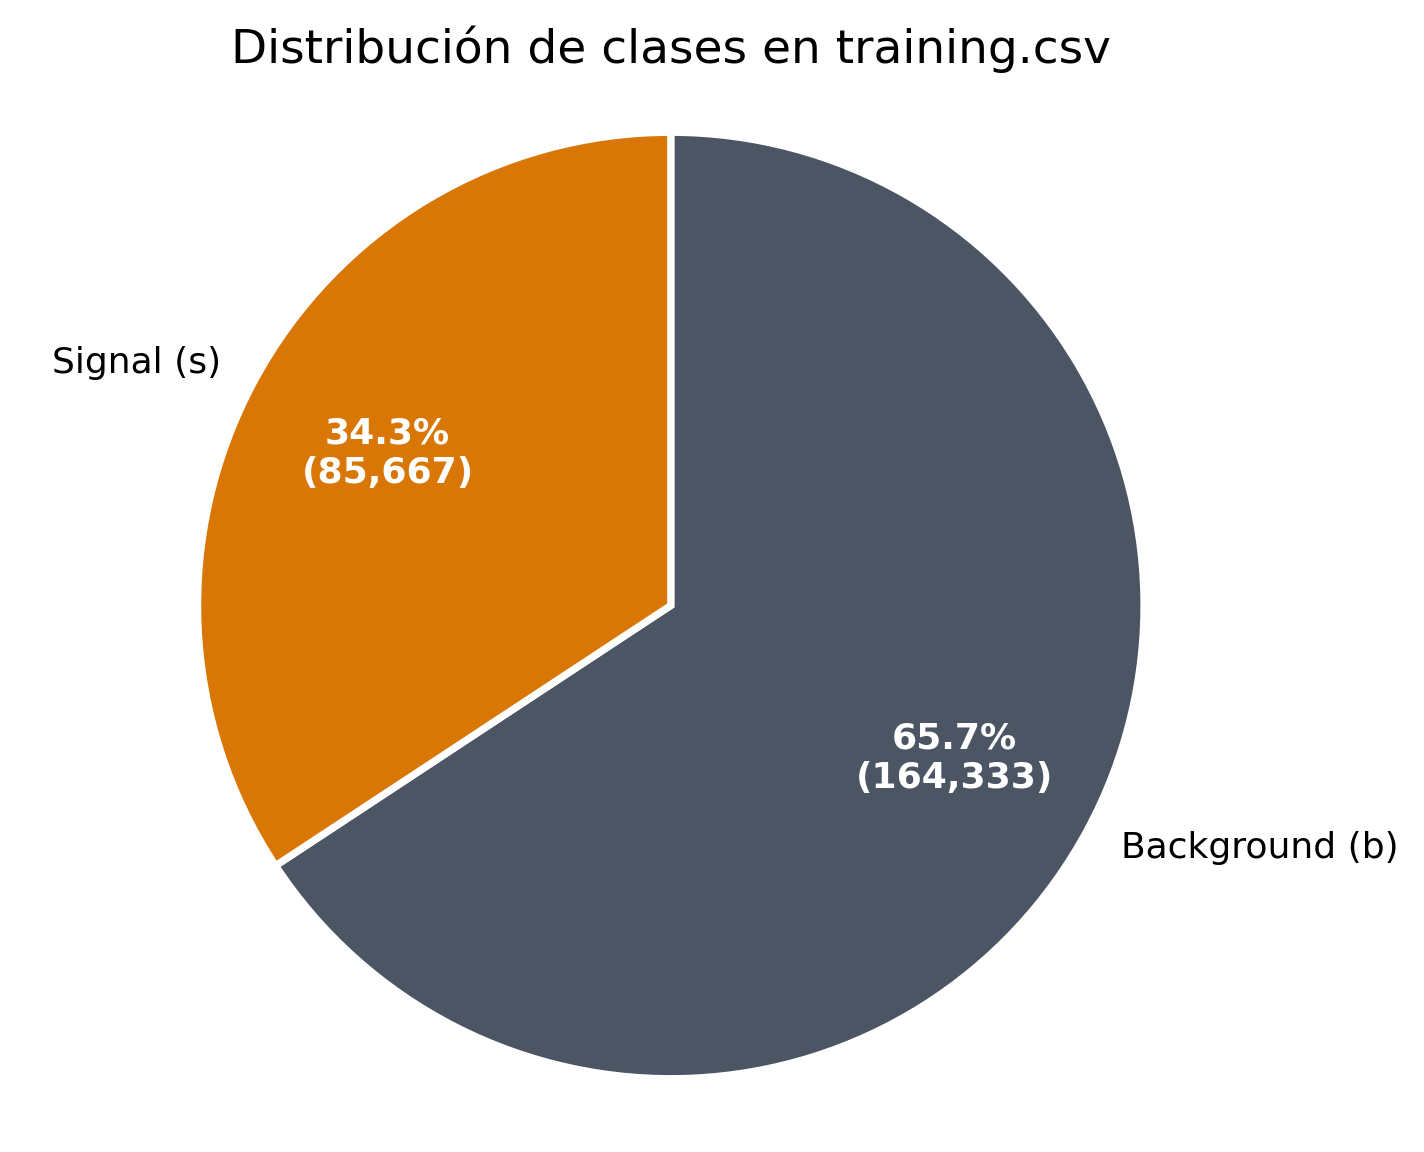
\includegraphics[width=0.52\textwidth]{img/fig_2_1_distribucion_clases.png}
    \caption{Distribución de la variable objetivo en el conjunto de entrenamiento.}
    \label{fig:distribucion-clases}
\end{figure}

\subsection{Valores faltantes y relación con jets}
Una particularidad importante del dataset es que los valores faltantes no aparecen codificados como nulos, sino con el valor artificial \texttt{-999}. Este valor no representa una medición física válida, sino una variable que no pudo calcularse o que no tiene sentido para cierto evento. Por este motivo, durante el análisis se lo trató como un marcador de faltante y no como un número real.

Los faltantes no se distribuyen de forma aleatoria. En gran parte están relacionados con la cantidad de jets del evento, representada por \texttt{PRI\_jet\_num}. Por ejemplo, si un evento no tiene jets, las variables asociadas al jet principal quedan indefinidas; si tiene menos de dos jets, las variables asociadas al segundo jet o al sistema de dos jets tampoco pueden calcularse. La Figura~\ref{fig:missing-jets} muestra esta relación: las variables como \texttt{PRI\_jet\_subleading\_pt}, \texttt{DER\_mass\_jet\_jet} y \texttt{DER\_deltaeta\_jet\_jet} presentan altos porcentajes de faltantes en los eventos con menos jets.

\begin{figure}[H]
    \centering
    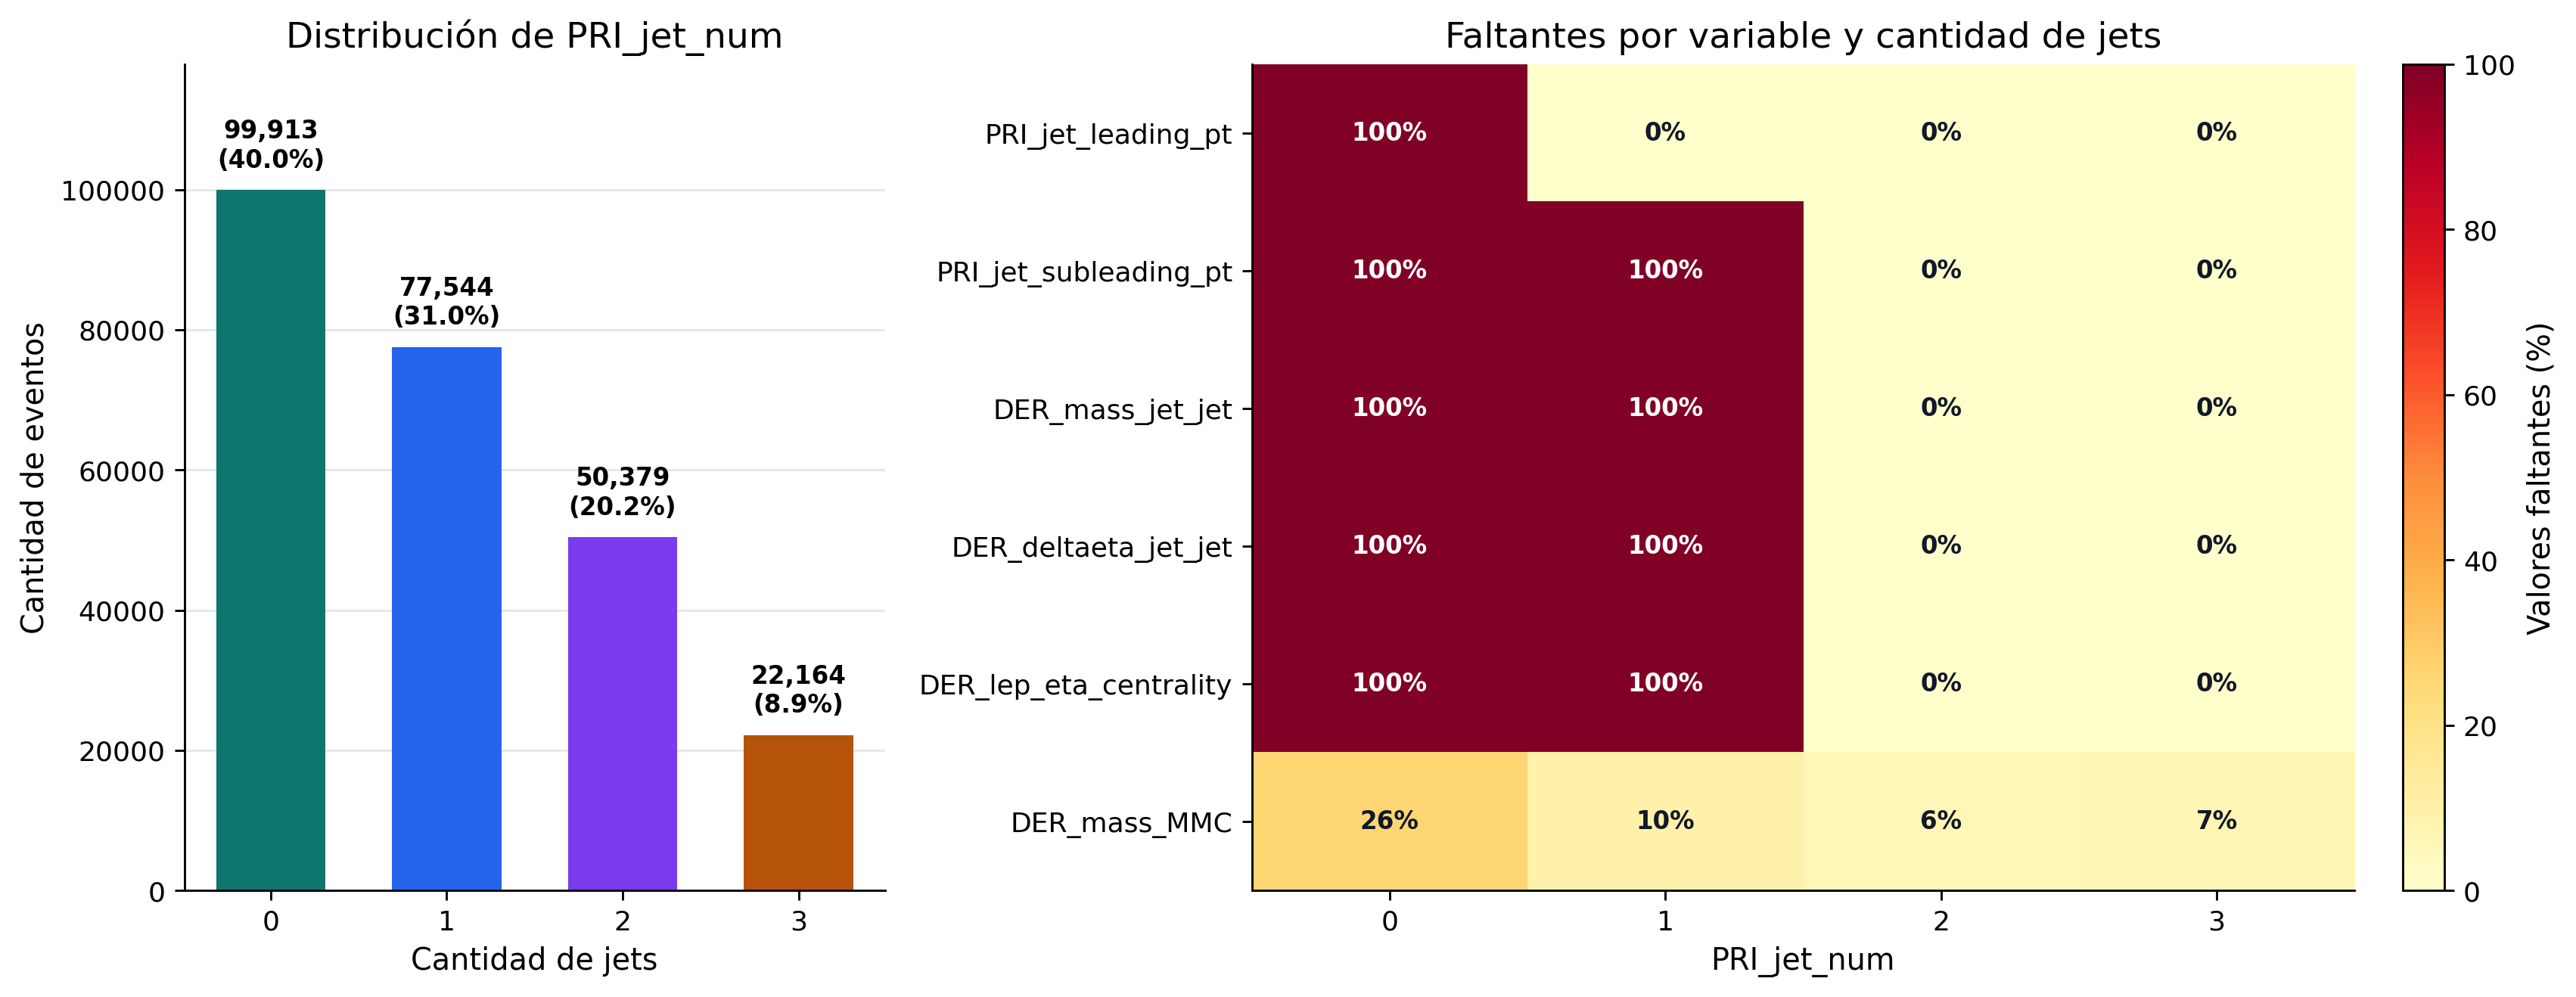
\includegraphics[width=0.94\textwidth]{img/fig_2_2_missing_y_jets.png}
    \caption{Distribución de eventos según \texttt{PRI\_jet\_num} y porcentaje de valores faltantes por variable y cantidad de jets.}
    \label{fig:missing-jets}
\end{figure}

\subsection{Variables físicas y análisis de \texttt{PRI\_jet\_num}}
Las variables del dataset se dividen principalmente en dos grupos. Las variables con prefijo \texttt{PRI\_*} corresponden a magnitudes primitivas medidas o reconstruidas directamente del evento, como momentos transversales, ángulos, energía faltante y cantidad de jets. Las variables con prefijo \texttt{DER\_*} son cantidades derivadas a partir de esas mediciones, como masas reconstruidas, separaciones angulares o relaciones entre objetos físicos.

Dentro de estas variables, \texttt{PRI\_jet\_num} resultó especialmente importante. Esta variable toma los valores 0, 1, 2 y 3, donde el valor 3 representa eventos con tres o más jets. No se trata de una magnitud continua, sino de una categoría que separa regímenes físicos distintos. Además, como se observó en la sección anterior, condiciona directamente qué variables pueden estar definidas. Por este motivo, en los preprocesamientos posteriores se decidió tratarla como variable categórica y no como una variable numérica ordinaria.

\subsection{Conclusiones para el preprocesamiento}
El análisis dio lugar a varias decisiones de preprocesamiento. En primer lugar, \texttt{EventId}, \texttt{Weight} y \texttt{Label} deben mantenerse fuera de la matriz de entrada \texttt{X}. En segundo lugar, el valor \texttt{-999} debe reemplazarse por \texttt{NaN} antes de aplicar transformaciones. Y que no conviene eliminar columnas por tener muchos faltantes, ya que estos contienen información estructural sobre el evento. Razon por la cual se consideró agregar indicadores de faltantes.

Y por otro lado, el análisis justifica dos acciones, tratar \texttt{PRI\_jet\_num} como categórica y construir variables físicas derivadas, como razones entre momentos, diferencias angulares y relaciones asociadas a jets.

\section{Preprocesamiento e ingeniería de características}
Luego de una primera etapa de pruebas exploratorias con distintos criterios de limpieza y transformación, se decidió reiniciar el preprocesamiento de forma más ordenada. El objetivo fue construir una base común reproducible, evitar fugas de información y comparar variantes bajo las mismas reglas. De esta forma, las diferencias observadas entre modelos podían atribuirse con mayor claridad al pipeline utilizado y no a cambios accidentales en la preparación de los datos.

\subsection{Procedimiento común de limpieza}
El procedimiento común se definió como una etapa previa a todos los pipelines. En esta etapa se separaron las columnas especiales \texttt{EventId}, \texttt{Label} y \texttt{Weight} de la matriz de entrada. La variable objetivo se codificó como un problema binario, con \texttt{0} para \textit{background} y \texttt{1} para \textit{signal}.

También se reemplazaron los valores \texttt{-999} por \texttt{NaN} inmediatamente después de cargar los datos. Esta transformación permitió que las etapas posteriores trabajaran con una representación explícita de los faltantes. Luego se realizó la separación entre entrenamiento y validación antes de ajustar cualquier transformación. Las medianas de imputación, los escaladores y los indicadores de faltantes se ajustaron únicamente con el conjunto de entrenamiento, evitando utilizar información del conjunto de validación.

Otro criterio importante fue no eliminar columnas por cantidad de datos faltantes al inicio. En lugar, se mantuvieron las variables originales, se agregaron indicadores de faltantes cuando correspondía y se guardaron tanto los datos procesados como los objetos de preprocesamiento ajustados. Esto hizo que los experimentos fueran más trazables y reproducibles.

\subsection{Pipelines de preprocesamiento evaluados}
Sobre la base común se construyeron distintas variantes para aislar el efecto de decisiones específicas: el tratamiento de \texttt{PRI\_jet\_num}, el tipo de escalado, la separación por regímenes de jets y la incorporación de variables derivadas. La Tabla~\ref{tab:pipelines-preprocesamiento} resume las variantes evaluadas.

\begin{table}[H]
    \centering
    \small
    \begin{tabular}{@{}p{0.12\textwidth} p{0.48\textwidth} p{0.28\textwidth}@{}}
        \toprule
        Pipeline & Idea principal & Objetivo \\
        \midrule
        \texttt{P00} & Logaritmos, imputación por mediana, \texttt{StandardScaler} e indicadores de faltantes. & Referencia inicial. \\
        \texttt{P01} & \texttt{P00} agregando one-hot encoding de \texttt{PRI\_jet\_num}. & Tratar la cantidad de jets como categórica. \\
        \texttt{P02} & \texttt{P01} usando \texttt{RobustScaler}. & Reducir sensibilidad a colas largas y outliers. \\
        \texttt{P03} & Preprocesamiento separado según grupos de jets. & Explotar regímenes físicos distintos. \\
        \texttt{P04} & \texttt{P02} más ingeniería de características físicas. & Enriquecer la representación del evento. \\
        \bottomrule
    \end{tabular}
    \caption{Resumen de los pipelines de preprocesamiento evaluados.}
    \label{tab:pipelines-preprocesamiento}
\end{table}

El pipeline \texttt{P00} se utilizó principalmente como referencia, mientras que \texttt{P01} y \texttt{P02} incorporaron el tratamiento categórico de \texttt{PRI\_jet\_num}. El pipeline \texttt{P03} evaluó una hipótesis diferente, entrenar transformaciones y modelos por separado para distintos grupos de jets. Finalmente, \texttt{P04} tomó la variante \texttt{P02} y le agregó variables derivadas físicamente motivadas.

\subsection{Feature engineering}
La ingeniería de características buscó hacer explícitas relaciones físicas que no siempre quedan representadas de forma directa por las variables originales. Las variables agregadas se agruparon en varias familias. Se incluyeron diferencias angulares entre objetos físicos, relaciones entre energía faltante y momento visible, razones de masas, proporciones asociadas a jets y balances entre el jet principal y el subprincipal. Cuando una característica derivada dependía de una variable indefinida, el resultado se mantuvo como \texttt{NaN} y fue tratado luego por el mismo mecanismo de imputación e indicadores de faltantes. Este enfoque permitió enriquecer el espacio de entrada sin romper la lógica del preprocesamiento común.

\subsection{Selección del pipeline final}
La comparación inicial mostró que \texttt{P04} era el pipeline más prometedor. En la evaluación con XGBoost sobre el split de validación, \texttt{P04} alcanzó el mejor AMS y el mejor AUC entre las variantes evaluadas. Además, también mejoró el desempeño de la red neuronal simple frente a pipelines sin ingeniería física.

El pipeline por grupos de jets, \texttt{P03}, resultó interesante, pero no superó a la alternativa global como estrategia principal. Por esta razón, se seleccionó \texttt{P04} como base para las etapas posteriores de modelado, validación cruzada y ajuste de hiperparámetros.

\section{Modelos evaluados y validación inicial}
\subsection{Modelos base considerados}
Una vez definidos los pipelines de preprocesamiento, se compararon distintas familias de modelos con el objetivo de elegir una línea principal de trabajo. La intención en esta etapa no fue optimizar cada modelo, sino obtener referencias comparables y evitar asumir desde el inicio que una única técnica sería la más adecuada.

Se consideraron modelos con distintos sesgos inductivos. La regresión logística se utilizó como baseline lineal, útil para medir cuánto podía capturarse con una frontera de decisión simple. Random Forest permitió evaluar un ensamble no lineal basado en árboles, sin recurrir todavía a boosting. XGBoost se incluyó como candidato fuerte para datos tabulares con interacciones no lineales. Finalmente, se entrenó una red neuronal densa simple para contrastar el desempeño de un modelo neuronal sobre los datos escalados.

Durante esta comparación se trabajó únicamente con datasets ya procesados y se mantuvo \texttt{Weight} fuera de la matriz de entrada. La métrica principal fue AMS, por ser la métrica relevante del desafío, y se utilizó AUC como medida auxiliar de la calidad del ranking producido por los scores.

\subsection{Primera comparación de pipelines y modelos}
La primera comparación cruzó los pipelines procesados con modelos base. Se evaluaron regresiones logísticas sobre \texttt{P00}, \texttt{P01} y \texttt{P02}; Random Forest sobre \texttt{P01} y \texttt{P02}; XGBoost base sobre \texttt{P01}, \texttt{P02} y \texttt{P04}; y una MLP simple sobre \texttt{P02} y \texttt{P04}. Se buscó separar el efecto del preprocesamiento del efecto de la familia de modelos.

Los modelos lineales quedaron claramente por debajo de los métodos basados en árboles y boosting, lo que indicó que una frontera lineal no era suficiente para capturar la estructura del problema. Random Forest mejoró respecto al baseline lineal, pero no quedó como candidato principal y presentó mayor costo de entrenamiento. La MLP simple fue competitiva, especialmente sobre \texttt{P04}, aunque no superó a XGBoost.

El mejor resultado inicial correspondió a \texttt{P04} + XGBoost base, con un AMS de 1.1129 y un AUC de 0.9102 en el split de validación. También se observó que \texttt{P01} y \texttt{P02} daban resultados muy similares con XGBoost, lo que sugiere que el tipo de escalado no era el factor dominante para los modelos de árboles. En cambio, la mejora de \texttt{P04} apuntaba a que las variables físicas derivadas aportaban información útil.

\subsection{Validación cruzada de candidatos}
A partir de la comparación inicial se redujo el conjunto de alternativas a cuatro candidatos representativos: \texttt{P04} + XGBoost base, \texttt{P02} + XGBoost base, \texttt{P04} + MLP simple y \texttt{P01} + Random Forest. Estos modelos se evaluaron mediante validación cruzada de 5 folds, manteniendo el mismo criterio de partición para comparar de forma más estable.

La Figura~\ref{fig:cv-candidatos-ams} resume el AMS medio y su variabilidad entre folds. El candidato \texttt{P04} + XGBoost obtuvo el mejor AMS medio, 1.6210, con AUC medio 0.9124. \texttt{P02} + XGBoost quedó muy cerca, con AMS medio 1.6143 y menor desvío, por lo que se mantuvo como referencia simple y estable. La MLP sobre \texttt{P04} resultó competitiva, pero no alcanzó a los modelos de boosting. Random Forest quedó como baseline robusto, aunque no justificó continuar con ajuste fino.

\begin{figure}[H]
    \centering
    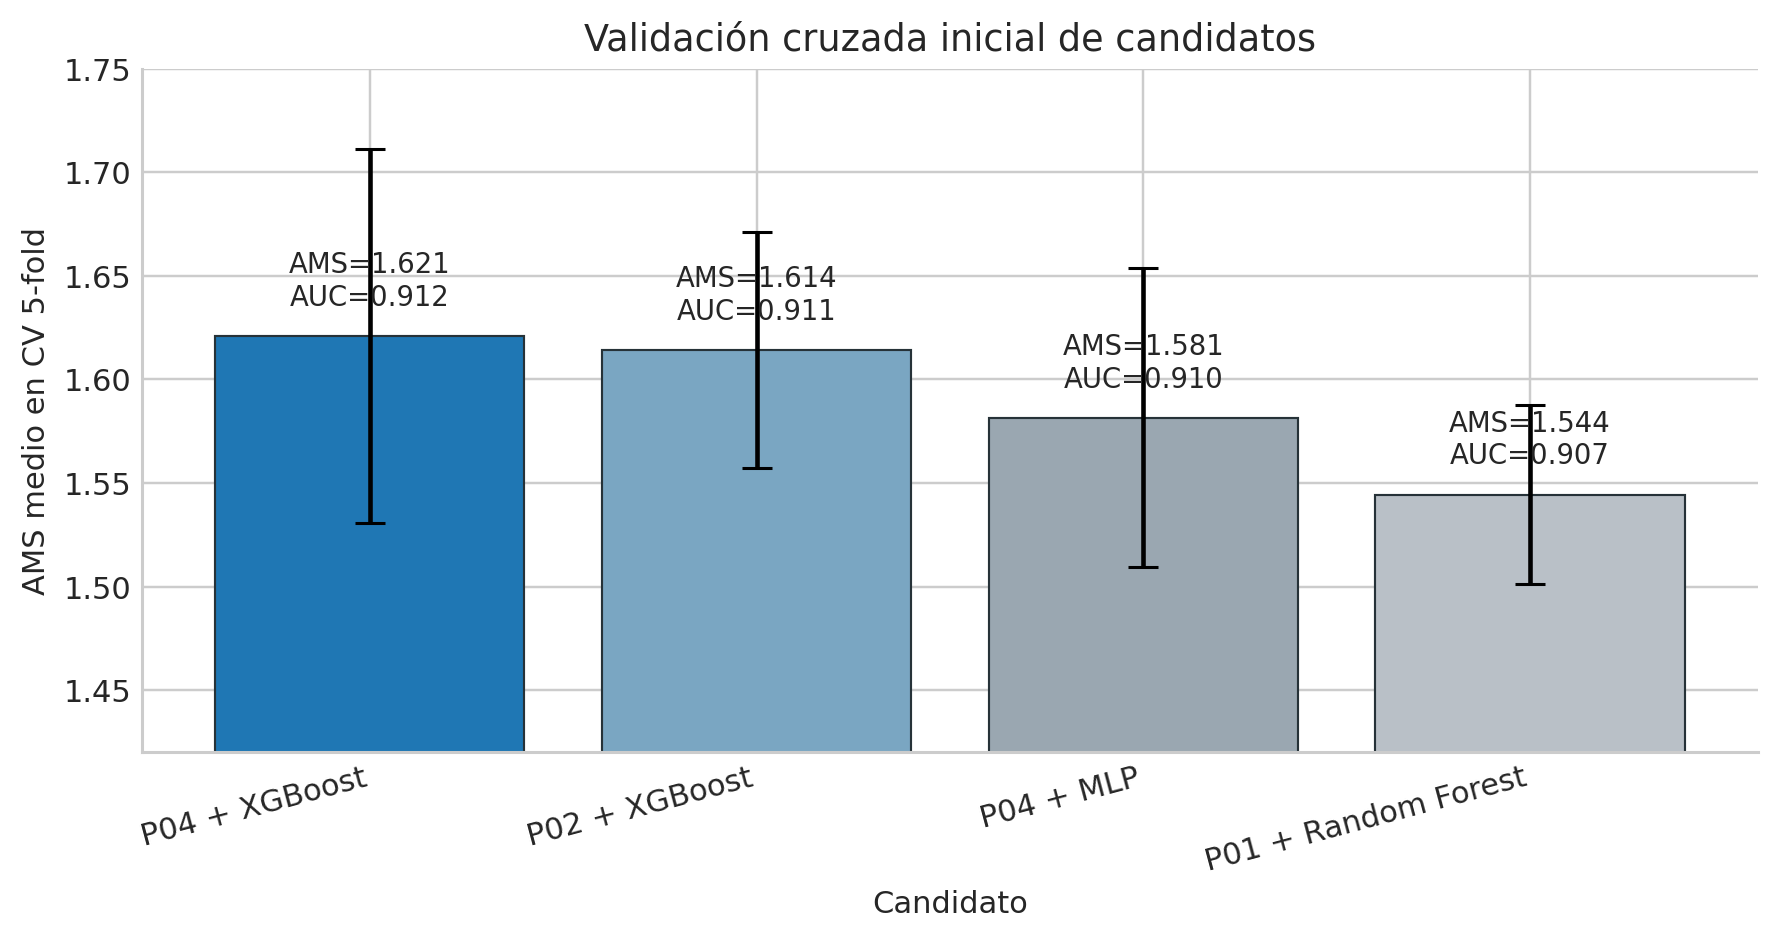
\includegraphics[width=0.78\textwidth]{img/fig_4_1_cv_candidatos_ams.png}
    \caption{Comparación por validación cruzada de candidatos iniciales. Las barras muestran el AMS medio en 5 folds y las líneas de error indican el desvío estándar.}
    \label{fig:cv-candidatos-ams}
\end{figure}

Esta validación permitió decidir la línea principal del trabajo. Aunque la diferencia entre \texttt{P04} y \texttt{P02} no fue grande, \texttt{P04} lideró en AMS medio y además era consistente con la hipótesis de incorporar información física derivada. Por esta razón, la búsqueda posterior se concentró en XGBoost sobre \texttt{P04}, manteniendo \texttt{P02} como referencia secundaria.

\section{Ajuste de hiperparámetros y regularización}
\subsection{Búsqueda incremental de hiperparámetros}

\subsection{Regularización del modelo}

\subsection{Uso de \texttt{sample\_weight}}

\subsection{Configuración final de XGBoost}

\section{Selección del punto de trabajo y submission final}
\subsection{Scores y política de decisión}

\subsection{Análisis OOF del threshold}

\subsection{Evaluación en Kaggle y ajuste del porcentaje}

\subsection{Submission final}

\section{Conclusiones}

\bibliographystyle{plain}
\bibliography{referencias} 
\end{document}
